% !TEX program = xelatex
\documentclass{article}
\usepackage{graphicx,geometry,hyperref,float}
% Justify Paragrapher
\newcommand{\justified}
{
	\tolerance=1
	\emergencystretch=\maxdimen
	\hyphenpenalty=10000
	\hbadness=10000
}


\graphicspath{ {./images/} }
%%%%%%%%%%%%%%%%%%%%%%%%%%%%%%%%%%%%%%%%%%%%%%%%%%%%%%%%

\title{
	\vspace{4cm}
	\textbf{Data And Information Quality Project Report}\\
}
\author{}
\date{}

\begin{document}
\maketitle
\vfill
\justified
\begin{itemize}
	\item\textbf{PROJECT ID}: 21
	\item\textbf{PROJECT NUMBER}: 1
	\item\textbf{ASSIGNED DATASET}: USERS
	\item\textbf{STUDENT}: PASQUALE CASTIGLIONE 10657816
	\item\textbf{ASSIGNED TASK}: CLUSTERING
\end{itemize}

\newpage

\tableofcontents

\newpage



\section{SETUP CHOICES}

\subsection{Imputation}

\subsubsection{Simple Imputation}
Because of the nature of the dataset, propagating values from valid cells to cells with missing values, seemed to be the best choice. In fact this method showed very good result with the original data, but applying it to a shuffled version of the dataset showed worse results.  

\subsubsection{Advanced Imputation}
\emph{K-Nearest Neighbors} was used as the advanced technique to impute missing value as it was able to spot similiarity between tuples and impute values accordingly. Compared to the simple imputation this method proved to be worse with the original dataset but more robust to shuffling.

\subsection{Clustering}

\subsubsection{K-Modes}
Because of the categorical nature of the data, \emph{K-Modes}\footnote{\url{https://github.com/nicodv/kmodes}} was the first choice. In order to select the best number of clusters, \emph{elbow method} analysis was performed.

\subsubsection{K-Means}
The second clustering techniques used was \emph{K-Means}, applied using Jaccard as distance measure. \emph{Elbow method} analysis was performed to find out the best number of clusters.

\newpage
\section{PIPELINE IMPLEMENTATION}

	\subsection{Data Load and Dirty Dataset Generation:} First of all the dataset was loaded and, using the provided script, dirty datasets with different completeness levels were generated.
	\subsection{Data Exploration:} In this phase histograms of the datasets and heatmaps of the datasets with missing values were plotted in order to have a general idea of the data and to take decisions accordingly.
\begin{figure}[h]
	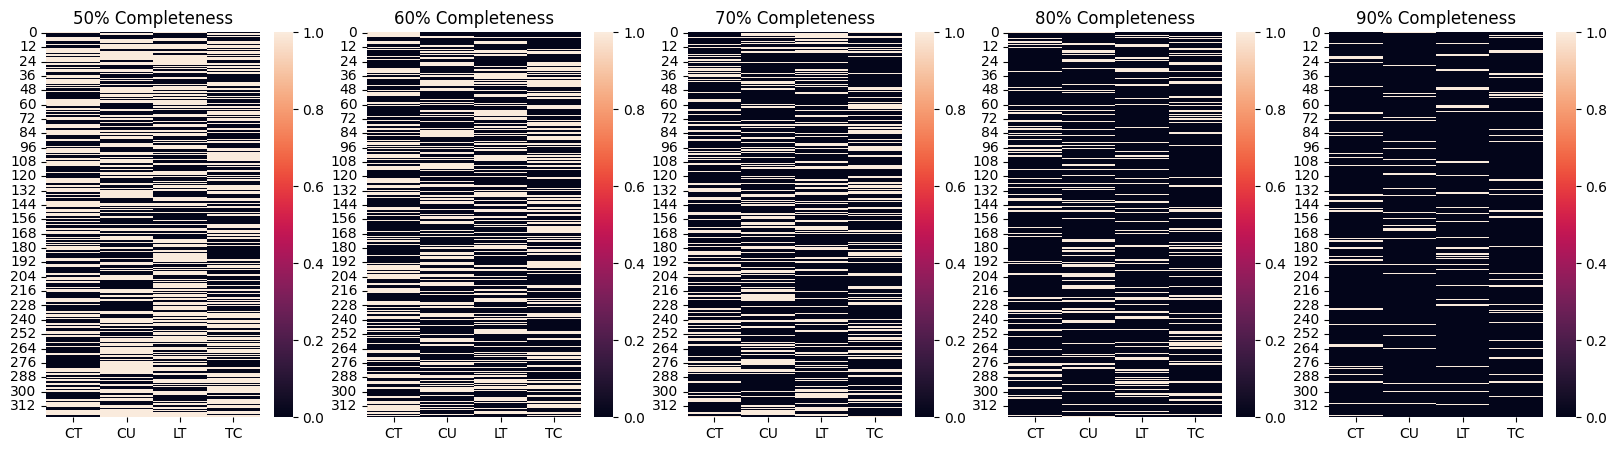
\includegraphics[width=\textwidth]{img/heatmaps.png}
	\caption{Null Values}
\end{figure}

\subsection{Imputation:}

\subsubsection{Simple Imputation:} For all the dirty datasets the method \texttt{fillna} was used. Firstly with the parameter \texttt{method='ffill'} and then with \texttt{method='bfill'} in order impute null values in the first row. After the imputation accuracies were computed.
\begin{figure}[h]\centering
	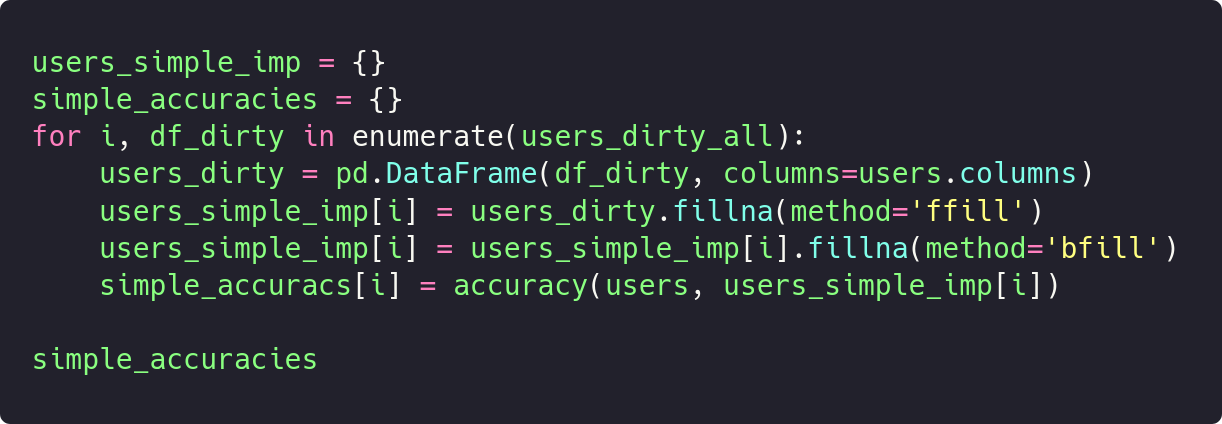
\includegraphics[scale=0.25]{img/simple.png}
	\caption{simple imputation}
\end{figure}
			
\subsubsection{Advanced Imputation:} First of all data was encoded as one hot arrays using the function \texttt{get\_dummies} from Pandas. Then \texttt{KNNImputer} from \emph{sklearn} was used to fit and transform the dirty datasets. After the imputation, data were decoded back to categorical. At the end accuracies were computed.
\begin{figure}[h]\centering
	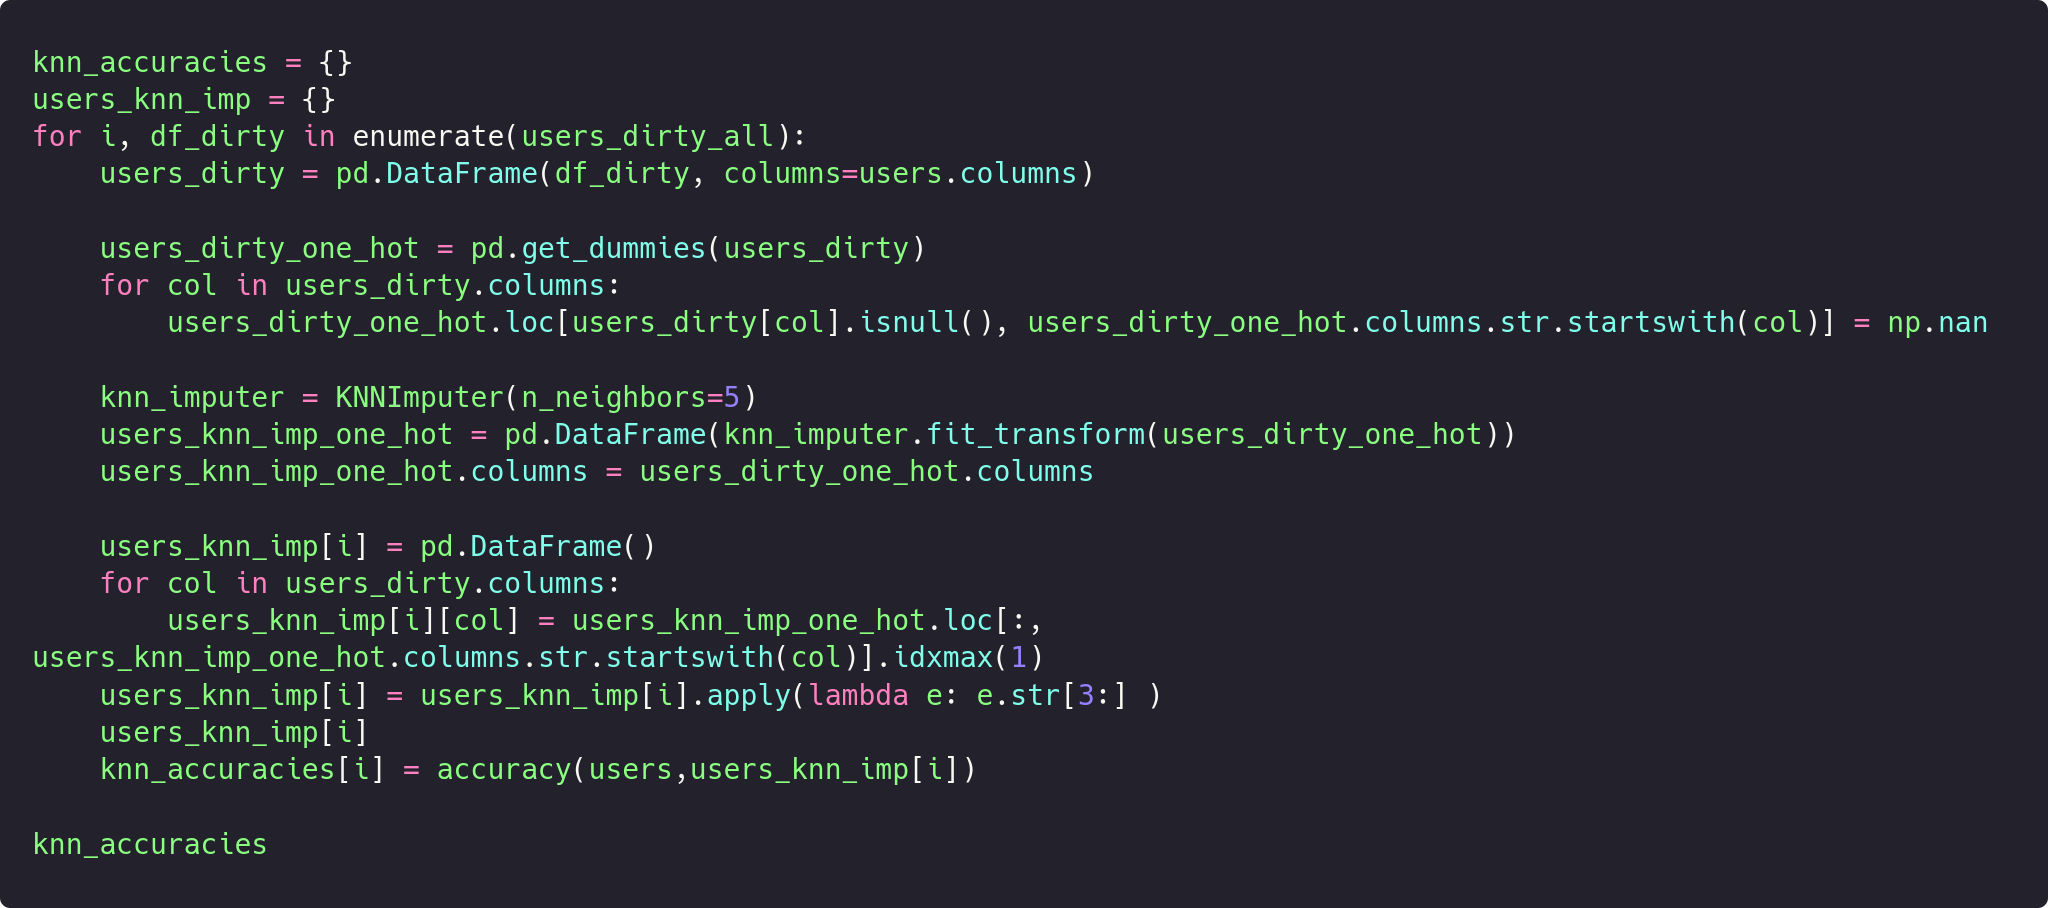
\includegraphics[scale=0.2]{img/knn_imputation.png}
	\caption{advanced imputation}
\end{figure}

\subsection{Clustering:}
			
\subsubsection{K-Modes:} First of all elbow analysis was performed to choose the number of clusters, after choosing it the model was fitted . In this phase \emph{cluster's centroids} were printed and a column with the assigned cluster was added to the dataframe
\begin{figure}[h]\centering
	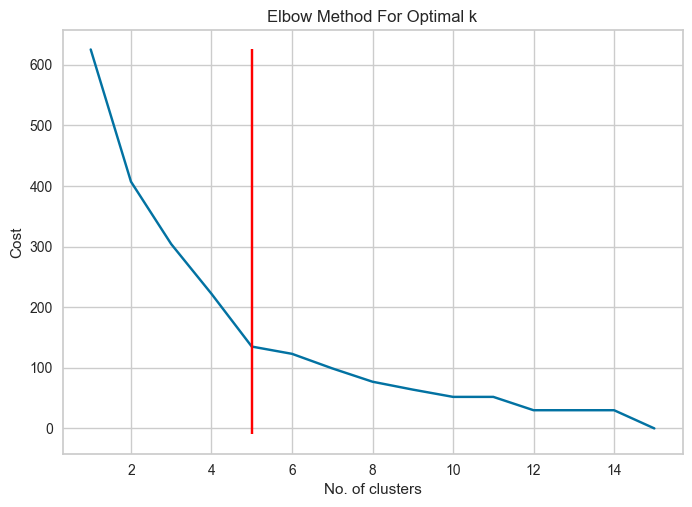
\includegraphics[scale=0.4]{img/elbow.png}
	\caption{Elbow Method for the original dataset}
\end{figure}
\begin{figure}[h]\centering
	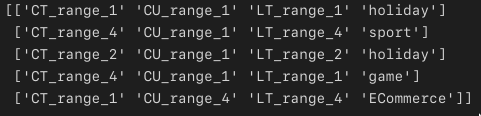
\includegraphics[scale=0.5]{img/centroids.png}
	\caption{K-Modes Centroids}
\end{figure}
			
\subsubsection{K-Means:} First of all the distance matrix was computed using Jaccard as distance between tuples. Then the usual elbow plot was plotted in order to choose the best number of clusters. At the end a column with the assigned cluster was added to the dataframe.  To asses the quality of the clustering silhuette score was computed using the function \texttt{silhuette\_score} from sklearn.
\begin{figure}[h]
	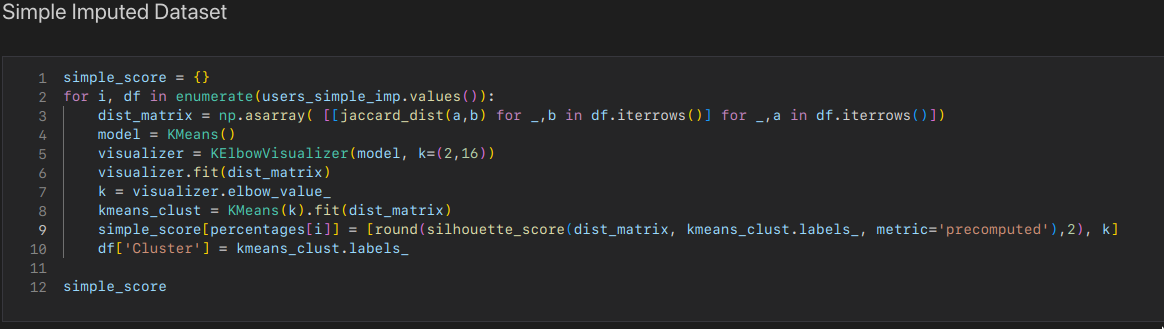
\includegraphics[width=\textwidth]{img/kmeans.png}
	\caption{K-Means on simple imputed datasets}
\end{figure}
\newpage
\section{RESULTS}

\subsection{Imputation}
To assess the quality of the imputation, accuracy was computed as the number of rows that were imputed as the original over all the rows.

\begin{figure}[h]\centering
	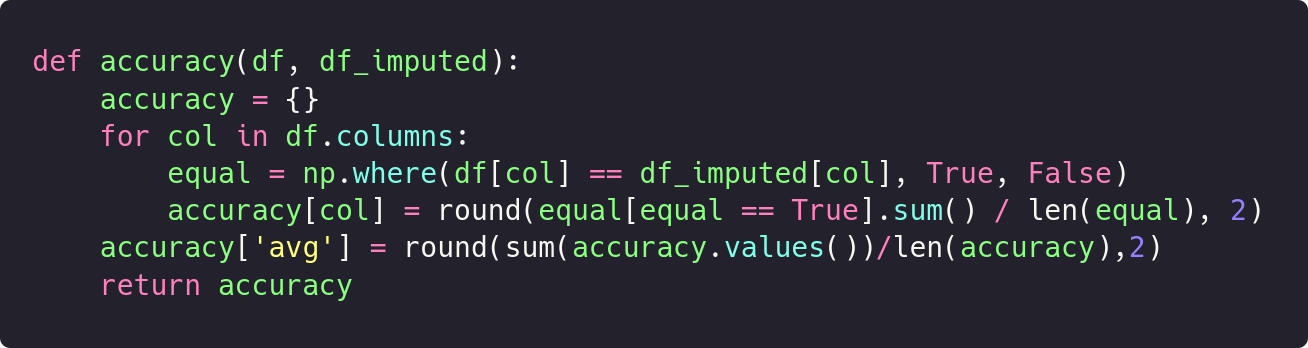
\includegraphics[scale=0.3]{img/accuracy.png}
	\caption{Function that compute the accuarcy}
\end{figure}
\subsubsection{Simple Imputation Accuracy}

\begin{table}[h]
\begin{minipage}{.45\textwidth}\centering
\begin{tabular}{cccccc}
			  & \textbf{CT} & \textbf{CU} & \textbf{LT} & \textbf{TC} & \textbf{avg} \\
\textbf{50\%} & 0.89        & 0.90        & 0.93        & 1.00        & 0.93 \\
\textbf{60\%} & 0.91        & 0.94        & 0.92        & 1.00        & 0.94 \\
\textbf{70\%} & 0.93        & 0.94        & 0.96        & 1.00        & 0.96 \\
\textbf{80\%} & 0.94        & 0.97        & 0.96        & 1.00        & 0.97 \\
\textbf{90\%} & 0.98        & 0.99        & 0.99        & 1.00        & 0.99
\end{tabular}
\caption{Simple Imputation}
\end{minipage}
\hfill
\begin{minipage}{.5\textwidth}\centering
\begin{tabular}{cccccc}
			  & \textbf{CT} & \textbf{CU} & \textbf{LT} & \textbf{TC} & \textbf{avg} \\
\textbf{50\%} & 0.67        & 0.83        & 0.64        & 0.66        & 0.70 \\
\textbf{60\%} & 0.69        & 0.89        & 0.74        & 0.72        & 0.76 \\
\textbf{70\%} & 0.80        & 0.90        & 0.80        & 0.78        & 0.82 \\
\textbf{80\%} & 0.84        & 0.92        & 0.87        & 0.85        & 0.87 \\
\textbf{90\%} & 0.93        & 0.97       & 0.95         & 0.93        & 0.94
\end{tabular}
\caption{Simple Imputation on Shuffled Dataset}
\end{minipage}
\end{table}

\subsubsection{Advanced Imputation Accuracy}
\begin{table}[h]
\begin{minipage}{.45\textwidth}\centering
\begin{tabular}{cccccc}
			  & \textbf{CT} & \textbf{CU} & \textbf{LT} & \textbf{TC} & \textbf{avg} \\
\textbf{50\%} & 0.81        & 0.89        & 0.76        & 0.79        & 0.81 \\
\textbf{60\%} & 0.84        & 0.93        & 0.85        & 0.87        & 0.87 \\
\textbf{70\%} & 0.93        & 0.95        & 0.90        & 0.92        & 0.92 \\
\textbf{80\%} & 0.92        & 0.97        & 0.94        & 0.95        & 0.94 \\
\textbf{90\%} & 0.97        & 1.00        & 0.97        & 0.98        & 0.98
\end{tabular}
\caption{KNN Imputation}
\end{minipage}
\hfill
\begin{minipage}{.5\textwidth}\centering
\begin{tabular}{cccccc}
			  & \textbf{CT} & \textbf{CU} & \textbf{LT} & \textbf{TC} & \textbf{avg} \\
\textbf{50\%} & 0.75        & 0.92        & 0.75        & 0.78        & 0.80 \\
\textbf{60\%} & 0.87        & 0.93        & 0.84        & 0.88        & 0.88 \\
\textbf{70\%} & 0.88        & 0.95        & 0.91        & 0.92        & 0.92 \\
\textbf{80\%} & 0.94        & 0.97        & 0.94        & 0.95        & 0.95 \\
\textbf{90\%} & 0.98        & 0.99        & 0.98        & 0.99        & 0.99
\end{tabular}
\caption{KNN Imputation on Shuffled Dataset}
\end{minipage}
\end{table}

\subsection{Clustering}
\subsubsection{K-Means}
To asses the quality of k-means clustering \emph{silhuette score} was computed.\\
\textbf{Original Dataset}: 0.72, 5 clusters

\begin{table}[h]
\begin{minipage}{0.5\textwidth}\centering
\begin{tabular}{ccc}
              & \textbf{score} & \textbf{clusters} \\
\textbf{50\%} & 0.25                      & 6                           \\
\textbf{60\%} & 0.31                      & 5                           \\
\textbf{70\%} & 0.32                      & 6                           \\
\textbf{80\%} & 0.44                      & 5                           \\
\textbf{90\%} & 0.58                      & 5                          
\end{tabular}
\caption{Silhouette score for simple imputed datasets}
\end{minipage}
\hfill
\begin{minipage}{0.45\textwidth}\centering
\begin{tabular}{ccc}
              & \textbf{score} & \textbf{clusters} \\
\textbf{50\%} & 0.58                      & 6                           \\
\textbf{60\%} & 0.61                      & 5                           \\
\textbf{70\%} & 0.64                      & 5                           \\
\textbf{80\%} & 0.68                      & 5                           \\
\textbf{90\%} & 0.72                      & 5                          
\end{tabular}
\caption{Silhouette score for advanced imputed datasets}
\end{minipage}
\end{table}
\end{document}
